%************************************************
\chapter{Accelerated Chemical Reaction optimisation using Multi-Task Learning}\label{ch:mtbo} 
%************************************************
This chapter is based on the following paper:

\begin{quote}
    Taylor C*., \textbf{Felton K.}*, Wigh D., Jeraal M., Grainger R., Chessari G., Johnson C., Lapkin A. \textit{ACS Central Science}. "Accelerated Chemical Reaction optimisation using Multi-Task Learning." 2023.
    * Joint first authors.
\end{quote}
\textbf{My contribution}: I developed  the idea of applying multitask Bayesian optimisation (MTBO) to reaction optimisation, implemented the MTBO strategy in Summit and executed the benchmarking studies. All experimental work was completed by Dr Connor Taylor and is presented here to show MTBO in an experimental setting.

\section{Introduction}

% In recent years, there has been increased interest in the use of automated, self-optimizing continuous flow platforms for the optimisation of chemical processes \cite{Reizman2016a, Fabry2016, Fitzpatrick2016, CortesBorda2016}. These platforms use automated reactors and machine-learning algorithms to learn from previous experiments, and thereby choose future experiments that ultimately maximize yield and/or other process objectives. The use of self-optimizing platforms has arisen from the desire for faster reaction optimisation, improved process sustainability and cheaper overall process development. The use of these platforms aims to enhance the capabilities of the researcher by removing the need for repetitive and labor-intensive experimentation, allowing them to focus on more challenging tasks. By leveraging algorithms, the platforms utilize only minimal reaction material but gain the most process information possible, making their deployment in fine chemical and pharmaceutical industries very attractive \cite{Clayton2019, Clayton2020}.

Recent work has shown that Bayesian optimisation is a particularly powerful tool for self-optimisation applications \cite{Amar2019, Schweidtmann2018, Shields2021}. However, in all previous studies, each optimisation begins with no \textit{a priori} information about the chemical landscape for the reaction of interest. This protocol therefore requires initial experimental iterations whereby the algorithm is learning about the experimental design space, without any prior information on where the optimal reaction conditions may be. This initial exploration can be expensive in terms of both cost and time, particularly when there may already be data on the broad chemical transformation of interest from previous optimisation campaigns. \textit{General} well-performing reaction conditions can also be identified for particular reaction classes, as highlighted in recent work by Angello \textit{et al.} \cite{Angello2022}, but do not give optimal conditions for specific transformations and cannot account for important parameters such as specific reactor differences, solubility, reaction selectivity, differences in substrate functionality or further adjacent objectives (E-factor, purification, downstream processing etc.). The use of optimisation strategies for specific substrates in specific instances is therefore still important for determining optimal yields (or other process outputs).

This chapter shows the first real-world examples of leveraging previous reaction optimisation data for unseen chemical transformations using multi-task Bayesian optimisation (MTBO). The framework of MTBO, first introduced by Swerksy \textit{et al.} \cite{Swersky2013}, replaces the standard probabilistic model in Bayesian optimisation with a multi-task model. As these multi-task models can be trained on data from related tasks,  the model can therefore utilize data from previously conducted similar reactions - both from the laboratory and from the literature. In this work, I first explore and benchmark the use of MTBO in simulated studies and then, in collaboration with experimentalists, exploit the methodology to optimize several pharmaceutically relevant C-H activation reactions using an autonomous flow reactor platform. These experimental case studies were chosen to highlight the effectiveness of MTBO in a late-stage medicinal chemistry or early stage process development context context through efficient material usage. The MTBO algorithm utilized is integrated into Summit, which was introduced in Chapter \ref{ch:summit}, and represents a powerful data-driven optimisation technique that can utilize known reaction data and ultimately lead to savings in material, time and overall cost.

\section{Methods}

\subsection{Multitask Bayesian optimisation}

As shown in Figure \ref{fig:multitask_overview}a-b, MTBO changes the probabilistic model in BO.  MTBO replaces the commonly used GP with a multi-task GP that can learn the correlations between different tasks to enable better predictions. In our case, the tasks are chemical transformations from the same reaction class with varying substrates. I use the intrinsic model of coregionalization originally proposed by Bonilla et al. \cite{Bonilla2007}, which defines a multi-task kernel $k^{ICM}_{\theta}$ as the Kronecker product of standard GP kernel (the Matérn kernel in our case) and a task kernel $k^t_{\theta}$:
\begin{equation}
    k^{ICM}_{\theta}(x,x') = k^t_{\theta} \otimes  k_{\theta}(x,x')
\end{equation}
The task kernel $k^t_{\theta}$ is a $T \times T$ matrix of trainable parameters where $T$ is the number of tasks. These parameters represent the inter-task correlation, and in the case of reactions should represent reaction similarity. The parameters start with a prior of very little task correlation and are updated with evidence from the data; if there is strong covariance between the data from different tasks, this multi-task GP will assume the reactions are similar and the auxiliary data can be used to improve predictions on the main task.

\begin{figure}
    \centering
    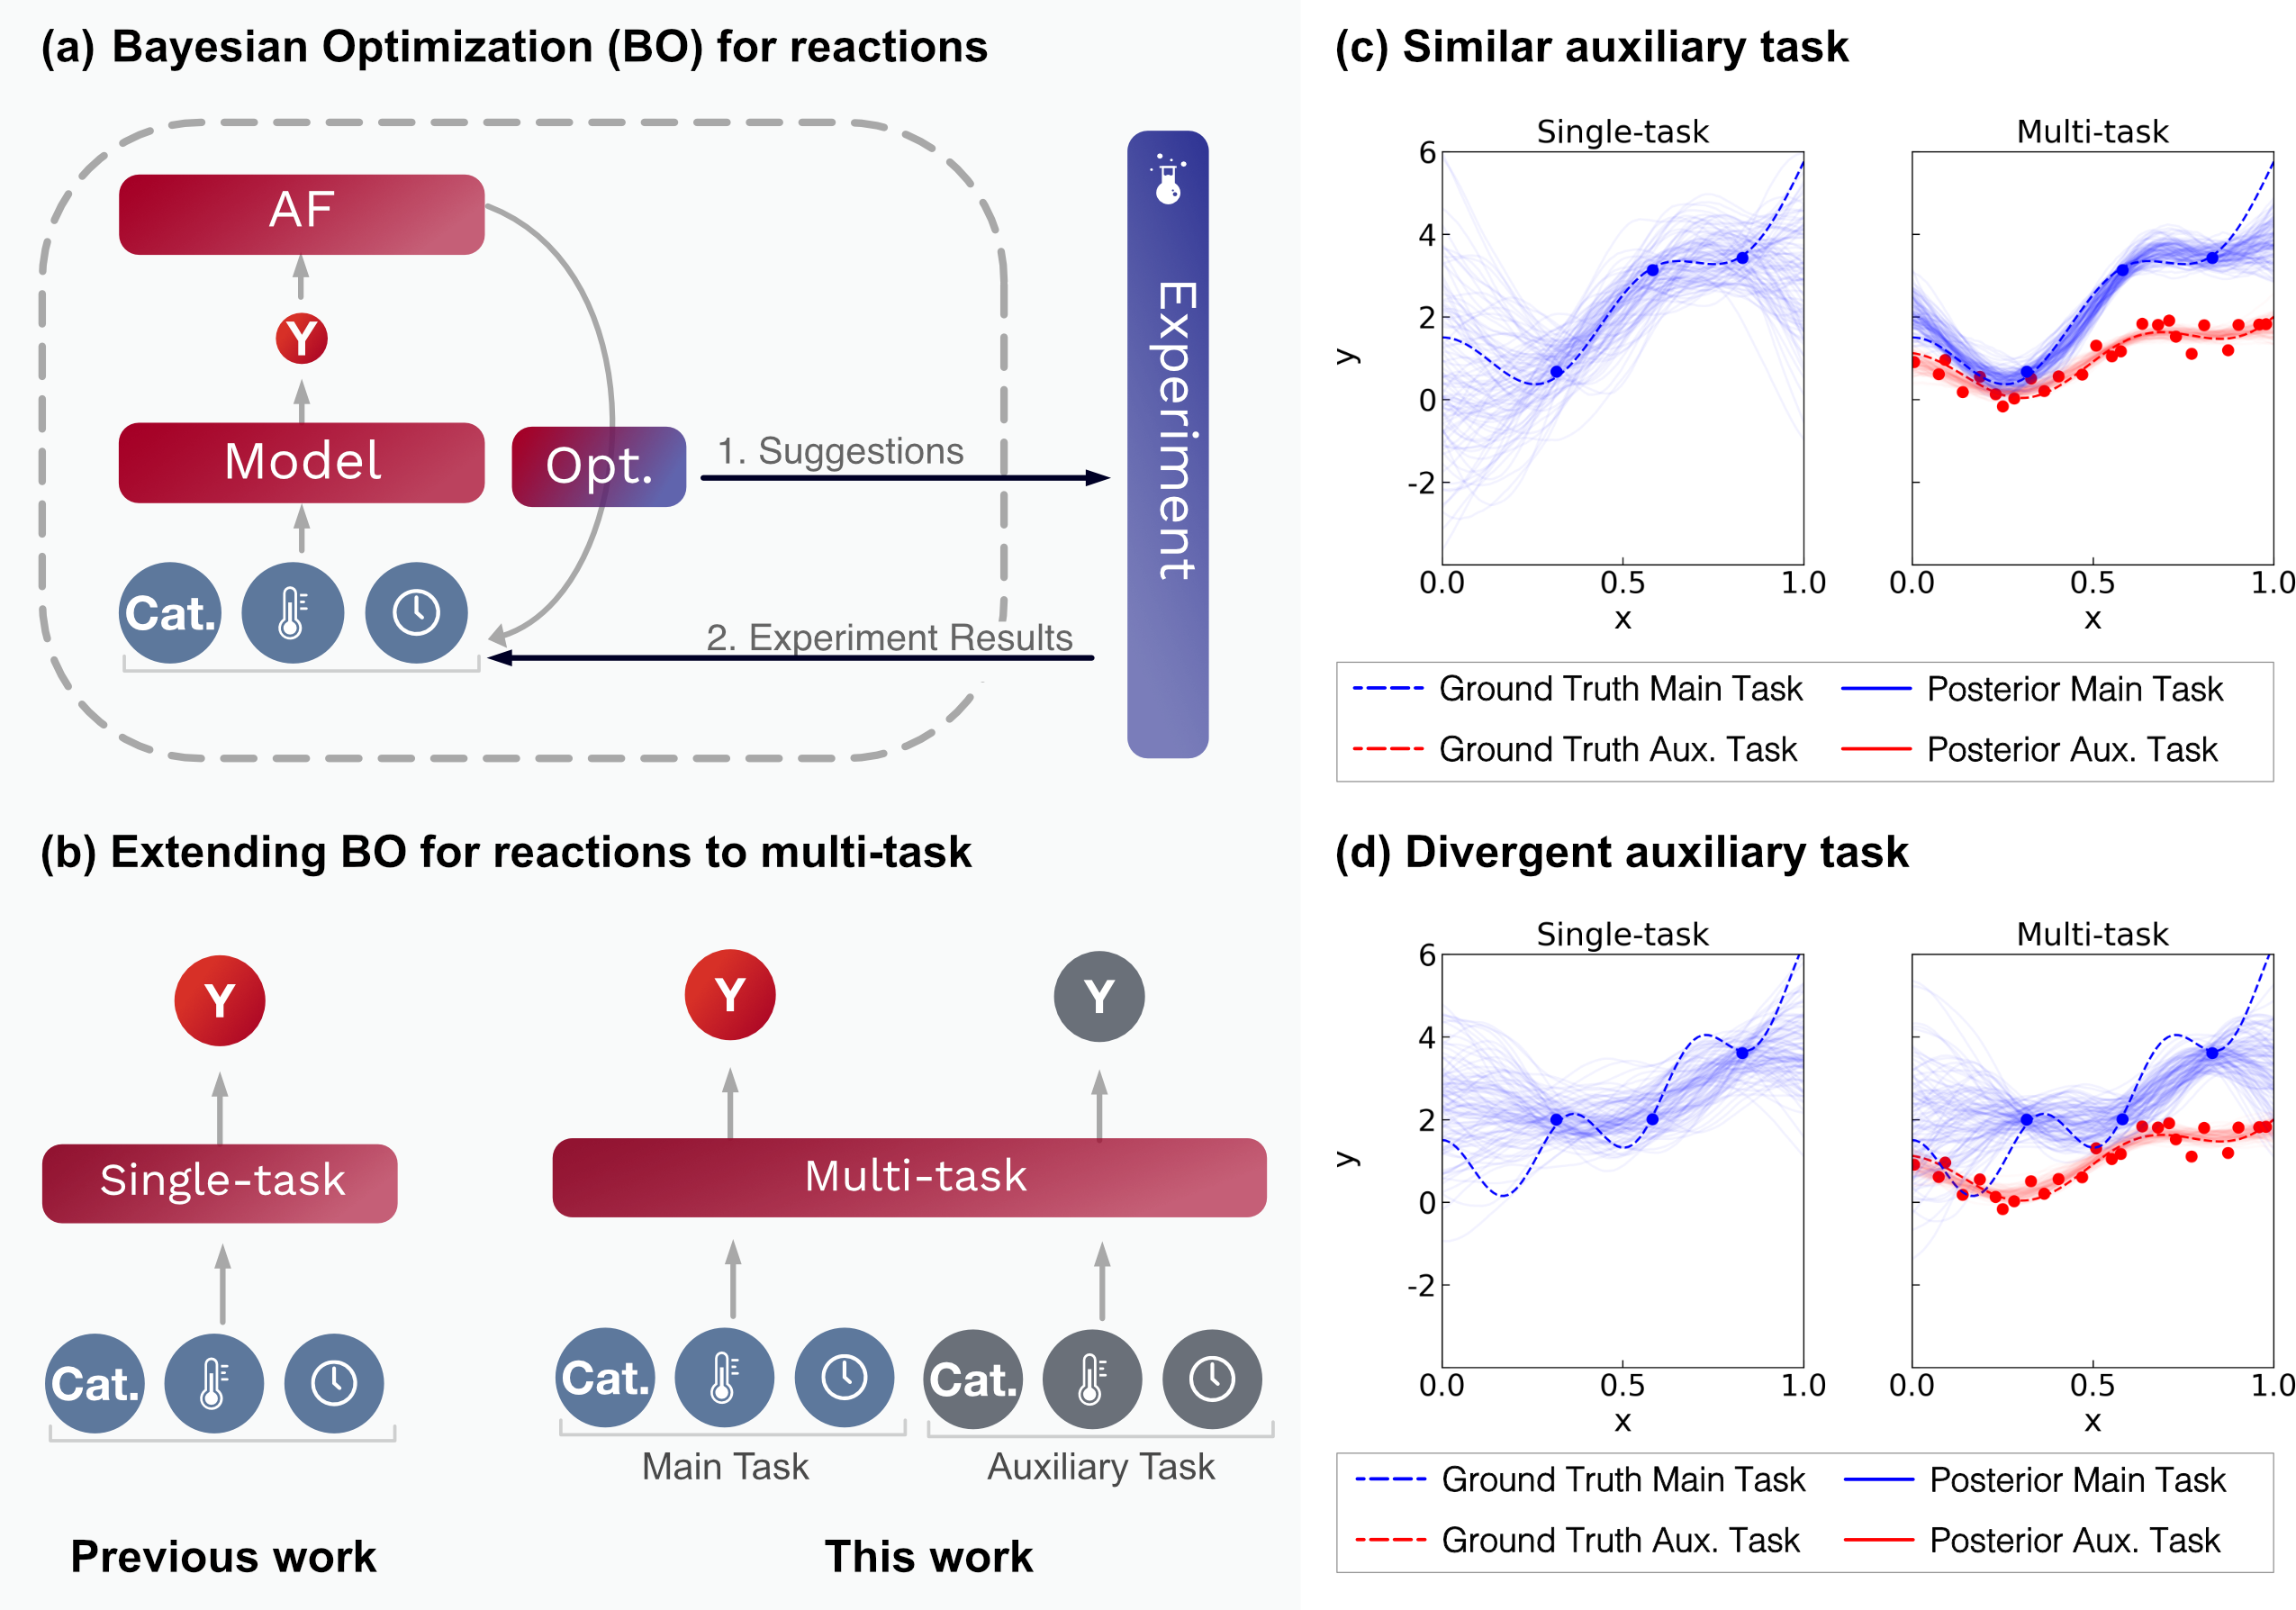
\includegraphics[width=1.2\textwidth]{gfx/Chapter04/paper_figure_1.png}
    \caption{A schematic description of multi-task Bayesian optimisation to the context of reaction optimisation. (a) Bayesian optimisation consists of a probabilistic model (typically a Gaussian process) that predicts experiment outputs (e.g. yield) given experiment conditions; an acquisition function (AF) that predicts the value of potential new experiments; and an optimisation algorithm (opt). (b) Multi-task Bayesian optimisation replaces the Gaussian process with a multi-task Gaussian process trained simultaneously on an auxiliary task. In our case, this auxiliary task is a similar reaction to the one being optimized, utilizing previous experimental results. (c) When the auxiliary task for a multi-task Gaussian process is similar to the main optimisation task, predictions on the main task are improved significantly. (d) When the auxiliary task for a multi-task Gaussian process is divergent to the main optimisation task, predictions on the main task are similar to what is observed for the baseline single-task Gaussian process.}
    \label{fig:multitask_overview}
\end{figure}

As a simple illustration of the benefits of multi-task GPs, I created example functions with one input and one output, then trained both a GP and multi-task GP on only three data points. In the multi-task GP case, we also generated 25 data points from an auxiliary task. As shown in Figure \ref{fig:multitask_overview}c, when the main and the auxiliary tasks are similar, the predictions from the multi-task GP (shown as samples from the posterior of the GP) more accurately represent the underlying function than the predictions from the single-task GP. The multi-task GP leverages the covariance between the data in the two tasks to improve predictions on the main task, even with limited data for the main task. As shown in Figure \ref{fig:multitask_overview}, when the main and the auxiliary tasks are divergent, predictions from the single-task and multi-task GP are highly variable. However, this variability in the multi-task GP is still useful because the BO algorithm will explore to better capture the underlying distribution of the main task.

\subsection{Benchmarks}
% Prior to real experimentation, we wanted to understand the performance of MTBO in simulated studies. We examined two literature reports that contain experimental results from Suzuki-Miyaura coupling reactions \cite{Baumgartner2018, Reizman2016b}, and one report with results from a Buchwald-Hartwig cross-coupling[51] (demonstrated in the Supporting Information), building a predictive model for the reaction yield to behave as the ground-truth for simulated optimisation studies. Buchwald-Hartwig and Suzuki-Miyaura couplings are ubiquitous in the pharmaceutical and fine chemicals industries as they allow rapid construction of aromatic scaffolds through reactions with few impurities.[52] We therefore chose these reaction classes because of their high value and applicability to real-world scenarios. More details on benchmark training can be found in the Appendix.

I used literature data to benchmark our strategies \textit{in silico}. The challenge is that chemical data is often recorded in unstructured text documents such as journal publications and patents. While there are some conventions, each author is free to express the details of a chemical reaction as they wish. Such unstructured information is not amenable to most machine learning algorithms. Therefore, I designed a custom data extraction workflow, shown in Figure \ref{fig:ord_pipeline}, that converts unstructured data into benchmarks that can be used for comparing various strategies. I leveraged the Open Reaction Database (ORD) format as a common representation of reactions \cite{Kearnes2021}. I wrote converters from spreadsheet formats to ORD. Once the data was transformed into ORD, the data was loaded into local storage on disk, and, subsequently, the featurization step turned the ORD schema into a set of features that can be used for training a benchmark or a GP for Bayesian optimisation.

\begin{figure}[t]
    \centering
    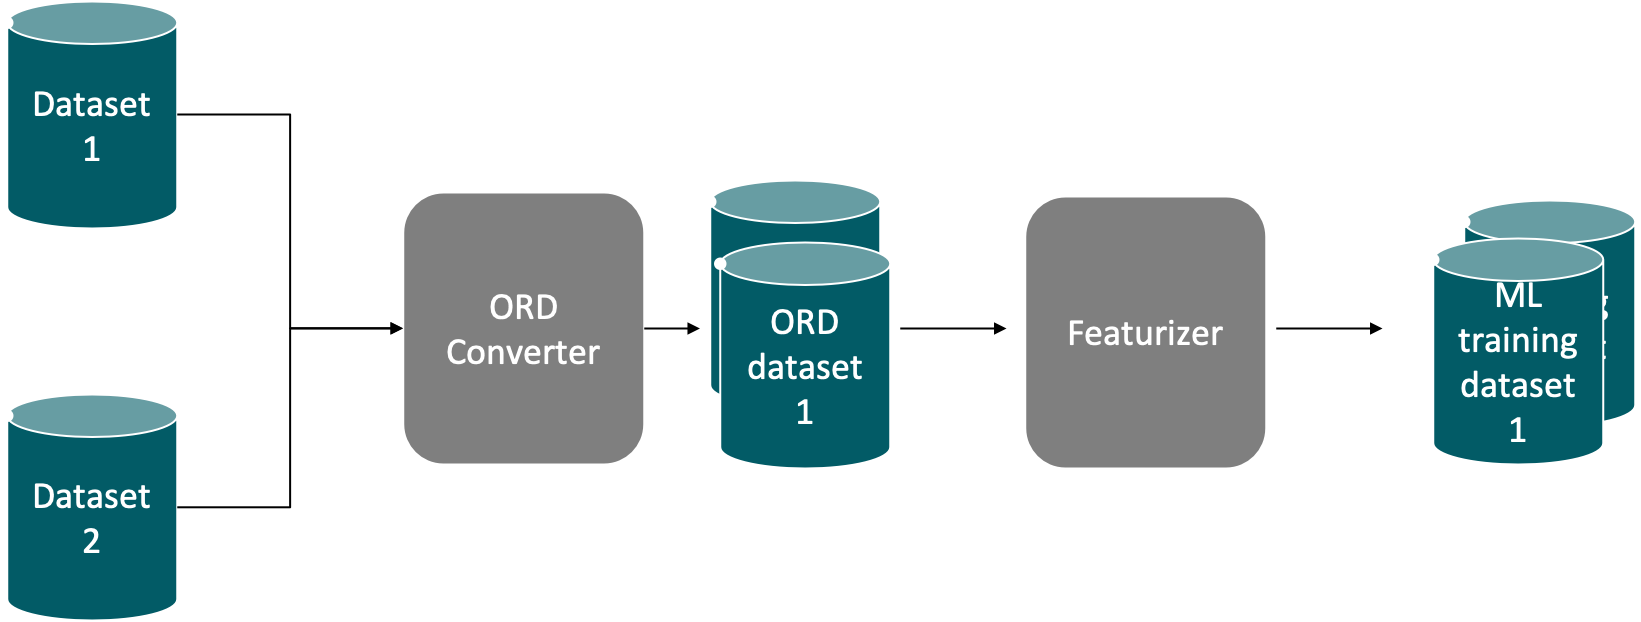
\includegraphics[width=\textwidth]{gfx/Chapter04/etl_pipeline.png}
    \caption{Diagram of a pipeline for turning raw data from the literature into a standard intermediate schema, which can be used to generate features for downstream machine learning tasks.}
    \label{fig:ord_pipeline}
\end{figure}

I examined two literature reports that contain experimental results from Suzuki-Miyaura coupling reactions \cite{Baumgartner2018, Reizman2016b} and one report with results from a Buchwald-Hartwig cross-coupling \cite{Baumgartner2019}. Buchwald-Hartwig and Suzuki-Miyaura couplings are ubiquitous in the pharmaceutical and fine chemicals industries as they allow rapid construction of aromatic scaffolds through reactions with few impurities \cite{Brown2016}. I therefore chose these reaction classes because of their high value and applicability to real-world scenarios. The specific reactions used are detailed in Figures \ref{fig:benchmarks_cn} and \ref{fig:benchmarks_suzuki}.


\begin{figure}
    \centering
    
\includegraphics[width=0.9\textwidth]{gfx/Chapter04/c_n_benchmarks_thesis.png}
    \caption{Benchmark examples of C-N cross coupling (C-N B1-B4) of nitrogen functionalized aromatics (1, 4, 6, 8) with p-tolyl triflate. Data is based on experiments by Baumgartner et al. 
 \cite{Baumgartner2019}. The base equivalents, temperature and reaction time, base and catalyst are varied to maximize yield.}
    \label{fig:benchmarks_cn}
\end{figure}

I leveraged Summit to build the predictive models from the literature reports. I utilized the ExperimentalEmulator feature in Summit (see Chapter \ref{ch:summit}). The regressor used was a neural network with one hidden layer of 512 units with a ReLu activation function. A one-hot encoding was used for the pre-catalyst and ligand combinations. The neural networks were trained by five-fold cross validation over 1000 epochs using stochastic gradient descent. See the Appendix \ref{ch:benchmarking_appendix} for the parity plots for the benchmarks. 

\subsection{Flow Reactor Platform}

Please note that all experimental work was completed by Dr Connor Taylor. The reactor platform consisted of two Vapourtec R2 modules for controlling flow rates, a Vapourtec R4 reactor module for controlling reactor temperature, a Gilson GX-271 liquid handler for dispensing and collecting reaction material and LC-MS analytical equipment (Shimadzu/Waters) for reaction outcome determination. The Vapourtec R2 modules were connected using 30 cm sections of 1 mm ID stainless steel tubing and T-pieces, entering a Vapourtec stainless steel reactor (10 mL volume) and exiting via a 50-bar back pressure regulator and a 80 cm section of 1 mm ID stainless steel tubing to a switching valve. For each reaction, with the experimental conditions determined through LHS or algorithmically, the liquid handler dispensed 2 mL slugs of the starting material (in this case, the chloroacetanilide) pre-dissolved in the selected solvent into the sample loop for pump A - this solution also contains biphenyl as an internal standard. The selected catalyst/ligand combination in the same solvent was then loaded into the sample loop for pump B, and the solvent of interest is loaded into pump C for dilution. The reaction was conducted with a constant 0.09 M reactor concentration, yielding the corresponding product (in this case, the oxindole), which was thereby analyzed utilizing a 4-way switching valve for on-line LC-MS. Using this methodology, experiments can be run using only minimal amounts of reaction material for each experiment as we were utilizing reaction slugs. This experimental workflow is illustrated in Figure \ref{fig:self_opt_setup}.

\begin{figure}
    \centering
    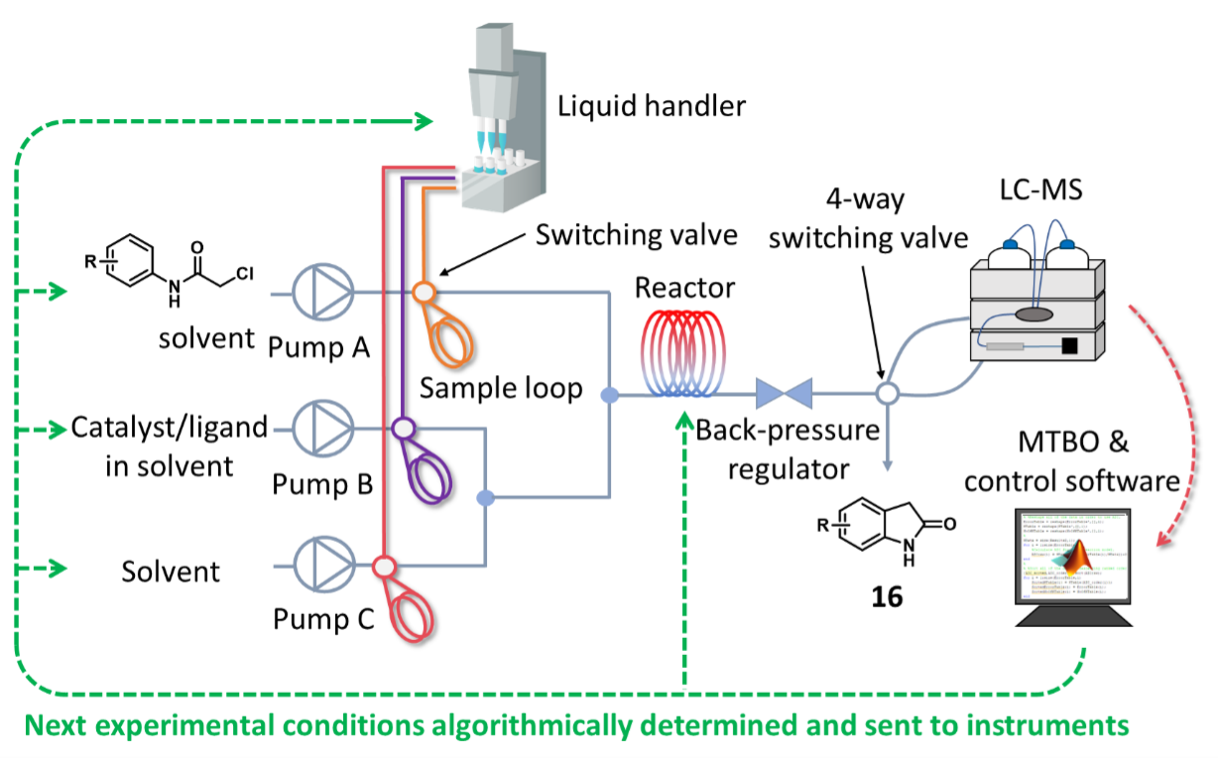
\includegraphics{gfx/Chapter04/self_optimization_setup.png}
    \caption{A schematic diagram of the experimental setup and protocol we used for the MTBO self-optimisation studies. Figure created by Connor Taylor.}
    \label{fig:self_opt_setup}
\end{figure}

\section{Results and Discussion}


\subsection{In Silico Case Studies: Suzuki-Miyaura Couplings}

I first executed \textit{in silico} MTBO studies using model chemical reactions as benchmarks. These models were generated using neural networks trained on literature experimental data that predict reaction yield. The model `Suzuki B1' was trained using Suzuki cross-coupling data from Baumgartner \textit{et al.} \cite{Baumgartner2018}, while the models `Suzuki R1-4' were trained using data from Reizman \textit{et al.} \cite{Reizman2016a}.  These specific transformations and the variables that affect these models are shown in Figure \ref{fig:benchmarks_suzuki}. When conducting benchmarking studies with MTBO, I initialized the optimization strategy using the best conditions from the auxiliary task.  I also included an additional baseline, STBO HS, that represents starting STBO with the best conditions from the auxiliary task(s) used for MTBO. This was done to understand how much of the acceleration of MTBO could be achieved by just using the optimal values from the auxiliary task.

\begin{figure}
    \centering
    
\includegraphics[width=0.9\textwidth]{gfx/Chapter04/suzuki_benchmarks_thesis.png}
    \caption{Reaction schemes for the Suzuki cross coupling benchmarks used in this chapter. The data for training the benchmarks are taken from Baumgartner et al. \cite{Baumgartner2018} and \cite{Reizman2016b}. Optimizing these reactions requires tuning continuous variables catalyst loading, reaction time and temperature as well as selecting from a library of Buchwald G3 catalysts \cite{Bruno2013}.}
    \label{fig:benchmarks_suzuki}
\end{figure}

Four specific case studies are highlighted in Figure \ref{fig:baumgartner_multitask}, each where the main task is Suzuki B1 and the auxiliary training task is one dataset from each of Suzuki R1-4. In each case study, a conventional single-task Bayesian optimisation (STBO) benchmark for the Suzuki B1 reaction serves as a comparison.   For each MTBO study, 96 datapoints from the auxiliary task were utilized. The average best yield for each algorithm is shown with a 95 \% confidence interval over 20 repeated runs. 

\begin{figure}
    \centering
    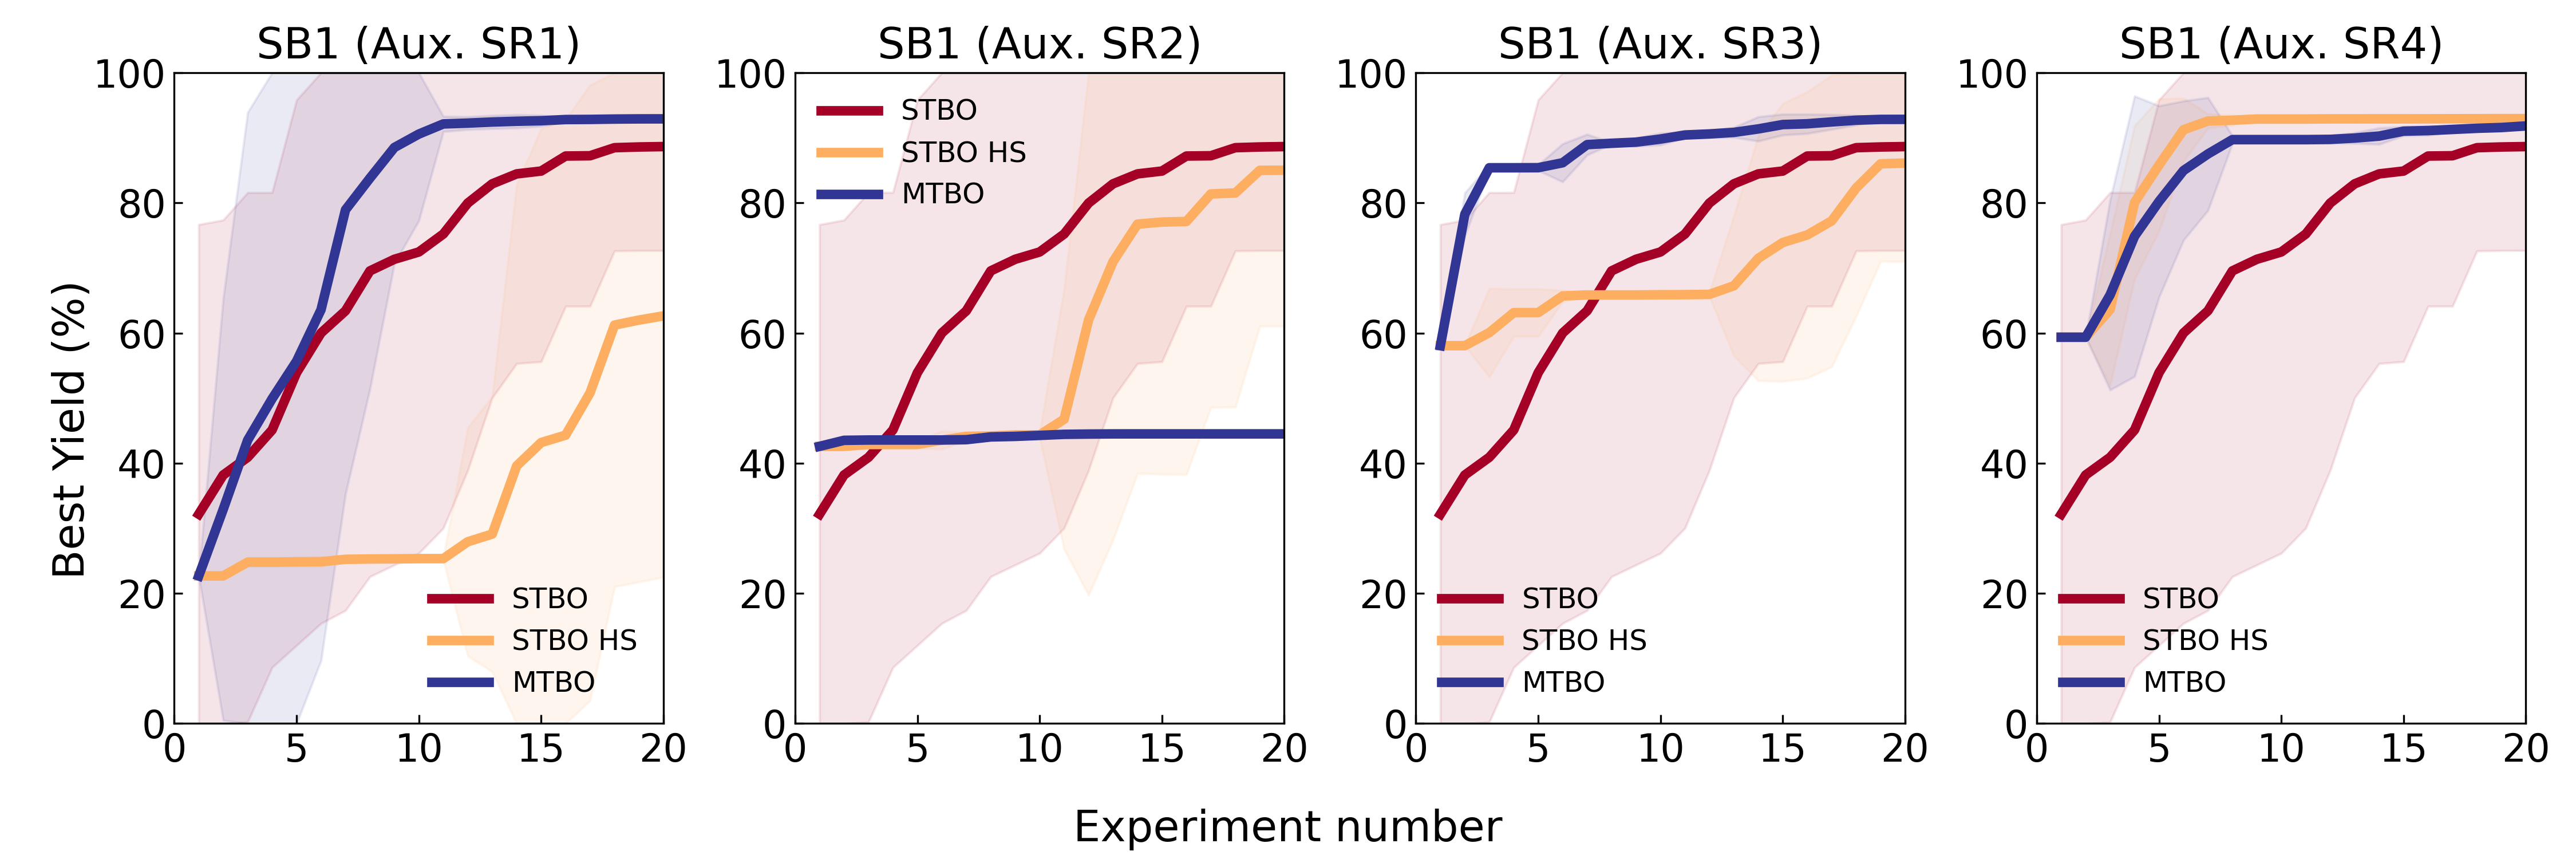
\includegraphics[width=1.2\textwidth]{gfx/Chapter04/baumgartner_suzuki_reizman_suzuki_one_cotraining_optimization.png}
    \caption{A comparison of the performance of single-task Bayesian optimisation (STBO) and multi-task Bayesian optimisation (MTBO) of Suzuki B1 with Suzuki R1-R4 as auxiliary tasks. The average best yield with a 95 \% confidence interval over 20 repeats is shown. The label above each plot refers to the auxiliary (Aux.) task based on the names in Figure \ref{fig:benchmarks_suzuki}, where Suzuki is abbreviated to S.}
    \label{fig:baumgartner_multitask}
\end{figure}

When leveraging Suzuki R1 as an auxiliary training task, MTBO initially suggested optimal conditions from the training task with P1-L4 (XantPhos). However, these give very low yields (25 \%) which leads to further exploration of the chemical space, resulting in optimal conditions with P1-L1 (XPhos) and a higher yield than STBO. The additional strength shown by MTBO in this case study is the greater speed in obtaining optimal results.

In the second case study, when the auxiliary task is Suzuki R2, MTBO appears to perform poorly, which is likely due to the low reactivity observed in Suzuki R2 and a noisy simulation benchmark. In this case, the best conditions from the training task also do not perform well on the main task, but the yield is moderate enough that it makes further exploration of the chemical space initially difficult in obtaining a better response. This suggests that MTBO may bias the training data in these circumstances when higher yields are possible but not expected, when given very low-yielding auxiliary tasks. 

To further investigate this issue, I plotted a measure of uncertainty calibration of the the single-task and multi-task GPs at each step in the optimisation. As shown in Figure  \ref{fig:uncertainty_multitask}, with more data, the single-task GP better calibrates the uncertainty of its predictions with the error on a holdout set of data, while the calibration of the multi-task model worsens. This suggests that the noise of the auxiliary task can have an affect on the uncertainty calibration of the multi-task model.

\begin{figure}
    \centering
    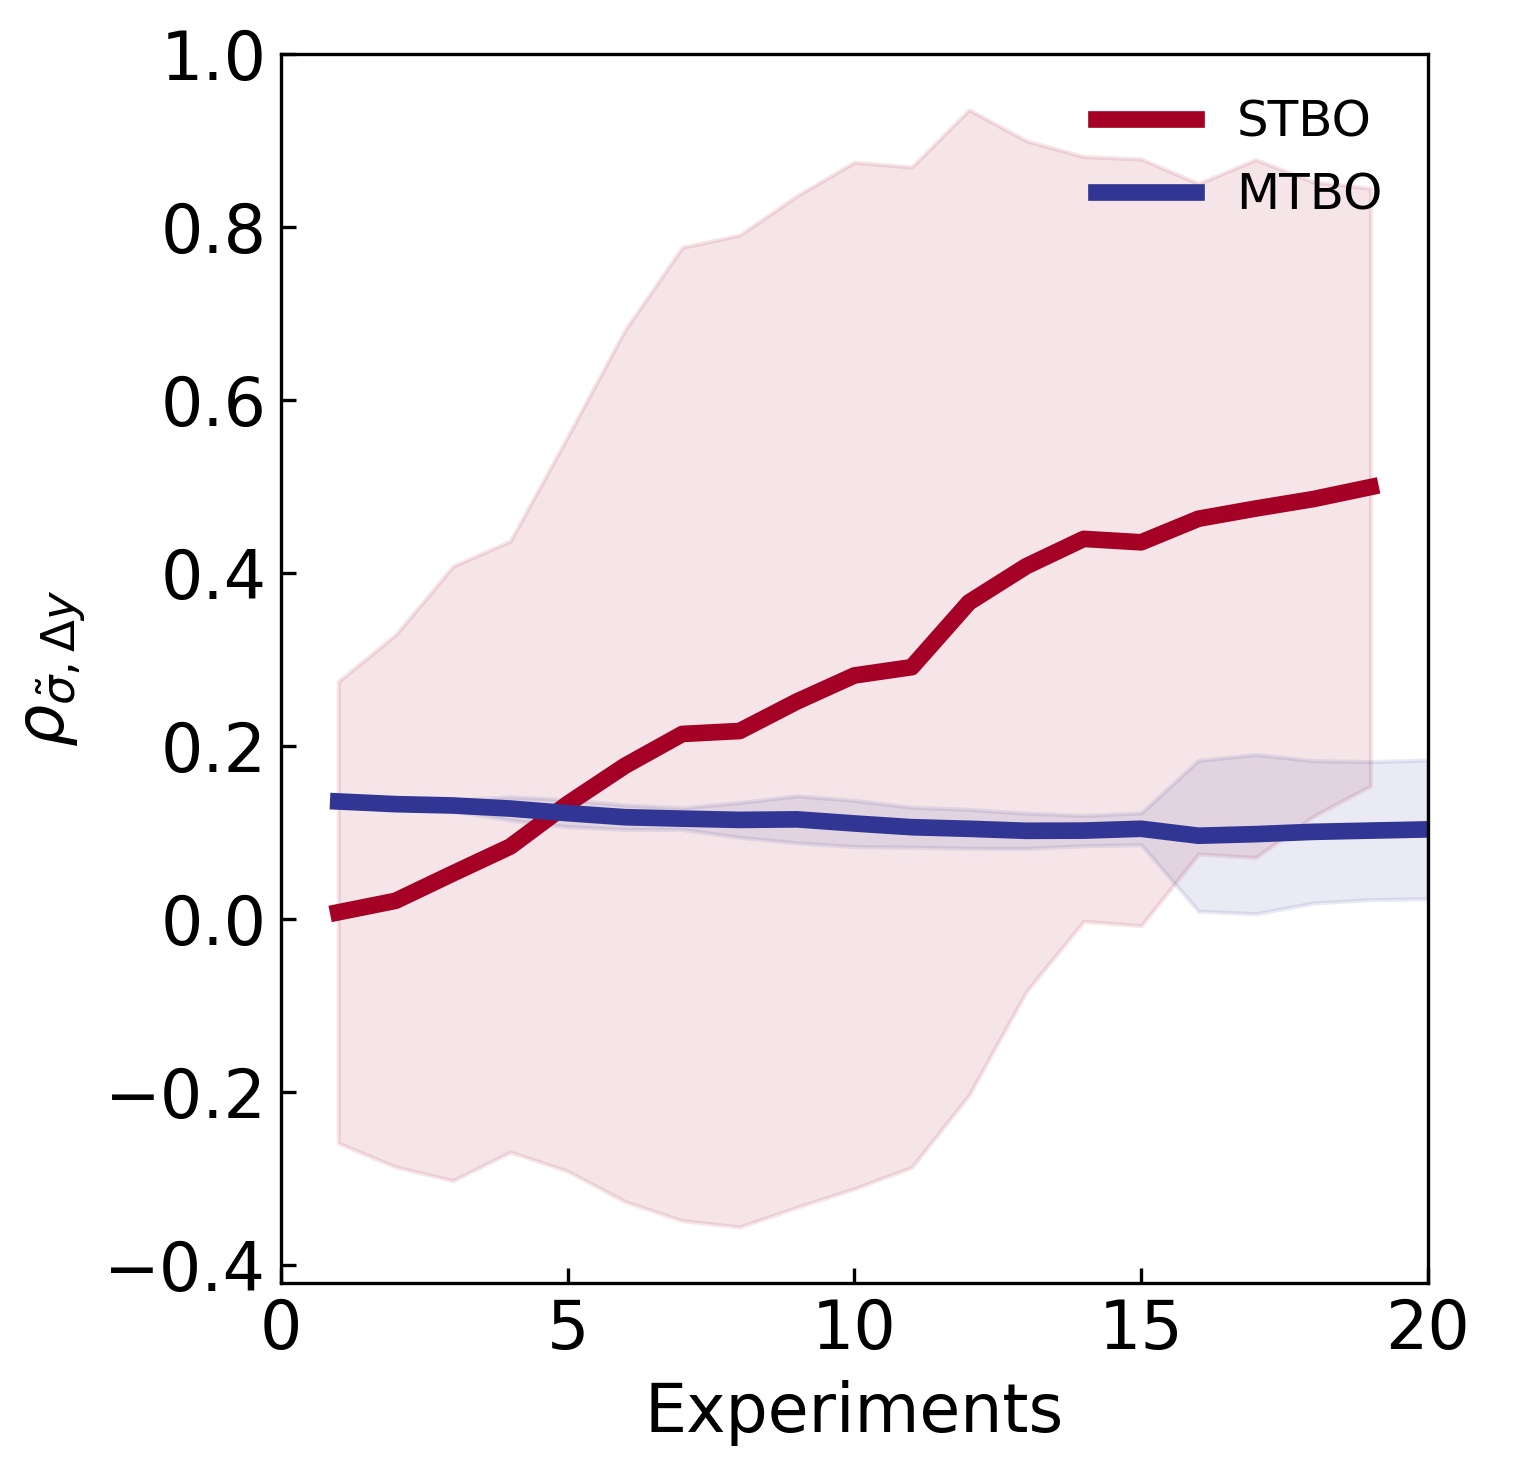
\includegraphics[width=0.6\textwidth]{gfx/Chapter04/baumgartner_suzuki_reizman_suzuki_case_2_optimization_uncertainty.png}
    \caption{Spearman's rank correlation coefficient ($\rho$) between standard deviation of predictions and absolute error on holdout set data. A higher value indicates a more calibrated model.}
    \label{fig:uncertainty_multitask}
\end{figure}


In the case studies where the auxiliary tasks were Suzuki R3-4, the reactivity of the substrates were much more similar in both the main and the training tasks, leading to similar optimal conditions being found. This means that MTBO achieved better, and much faster, results than STBO in these cases. 

STBO HS has variable performance relying heavily on the initial conditions provided. Overall, we observe that MTBO is less sensitive to changes in optima than MTBO, but MTBO is more sensitive to getting stuck in local optima that might be far away from the condition used initially. 

The performance of MTBO can be improved using \textit{multiple} auxiliary tasks. As shown in Figure \ref{fig:baumgartner_suzuki_reizman_suzuki_all_cotraining_optimisation}a, when Suzuki B1 is optimized with Suzuki R1-R4 as auxiliary tasks, the optimal conditions are always found by MTBO in fewer than five experiments. Both P1-L1 and P2-L1 are considered optimal for this reaction, and MTBO selects these two catalysts in over 80 \% of experiments during twenty repeats, when compared to \textless{} 50 \% frequency for STBO - this is highlighted in Figure \ref{fig:baumgartner_suzuki_reizman_suzuki_all_cotraining_optimisation}b. As MTBO utilizes optimal regions of chemical space that have been identified in previous tasks with similar reactivity, this allows the strategy to identify new (and better performing) optimal reaction conditions faster.

\begin{figure}
    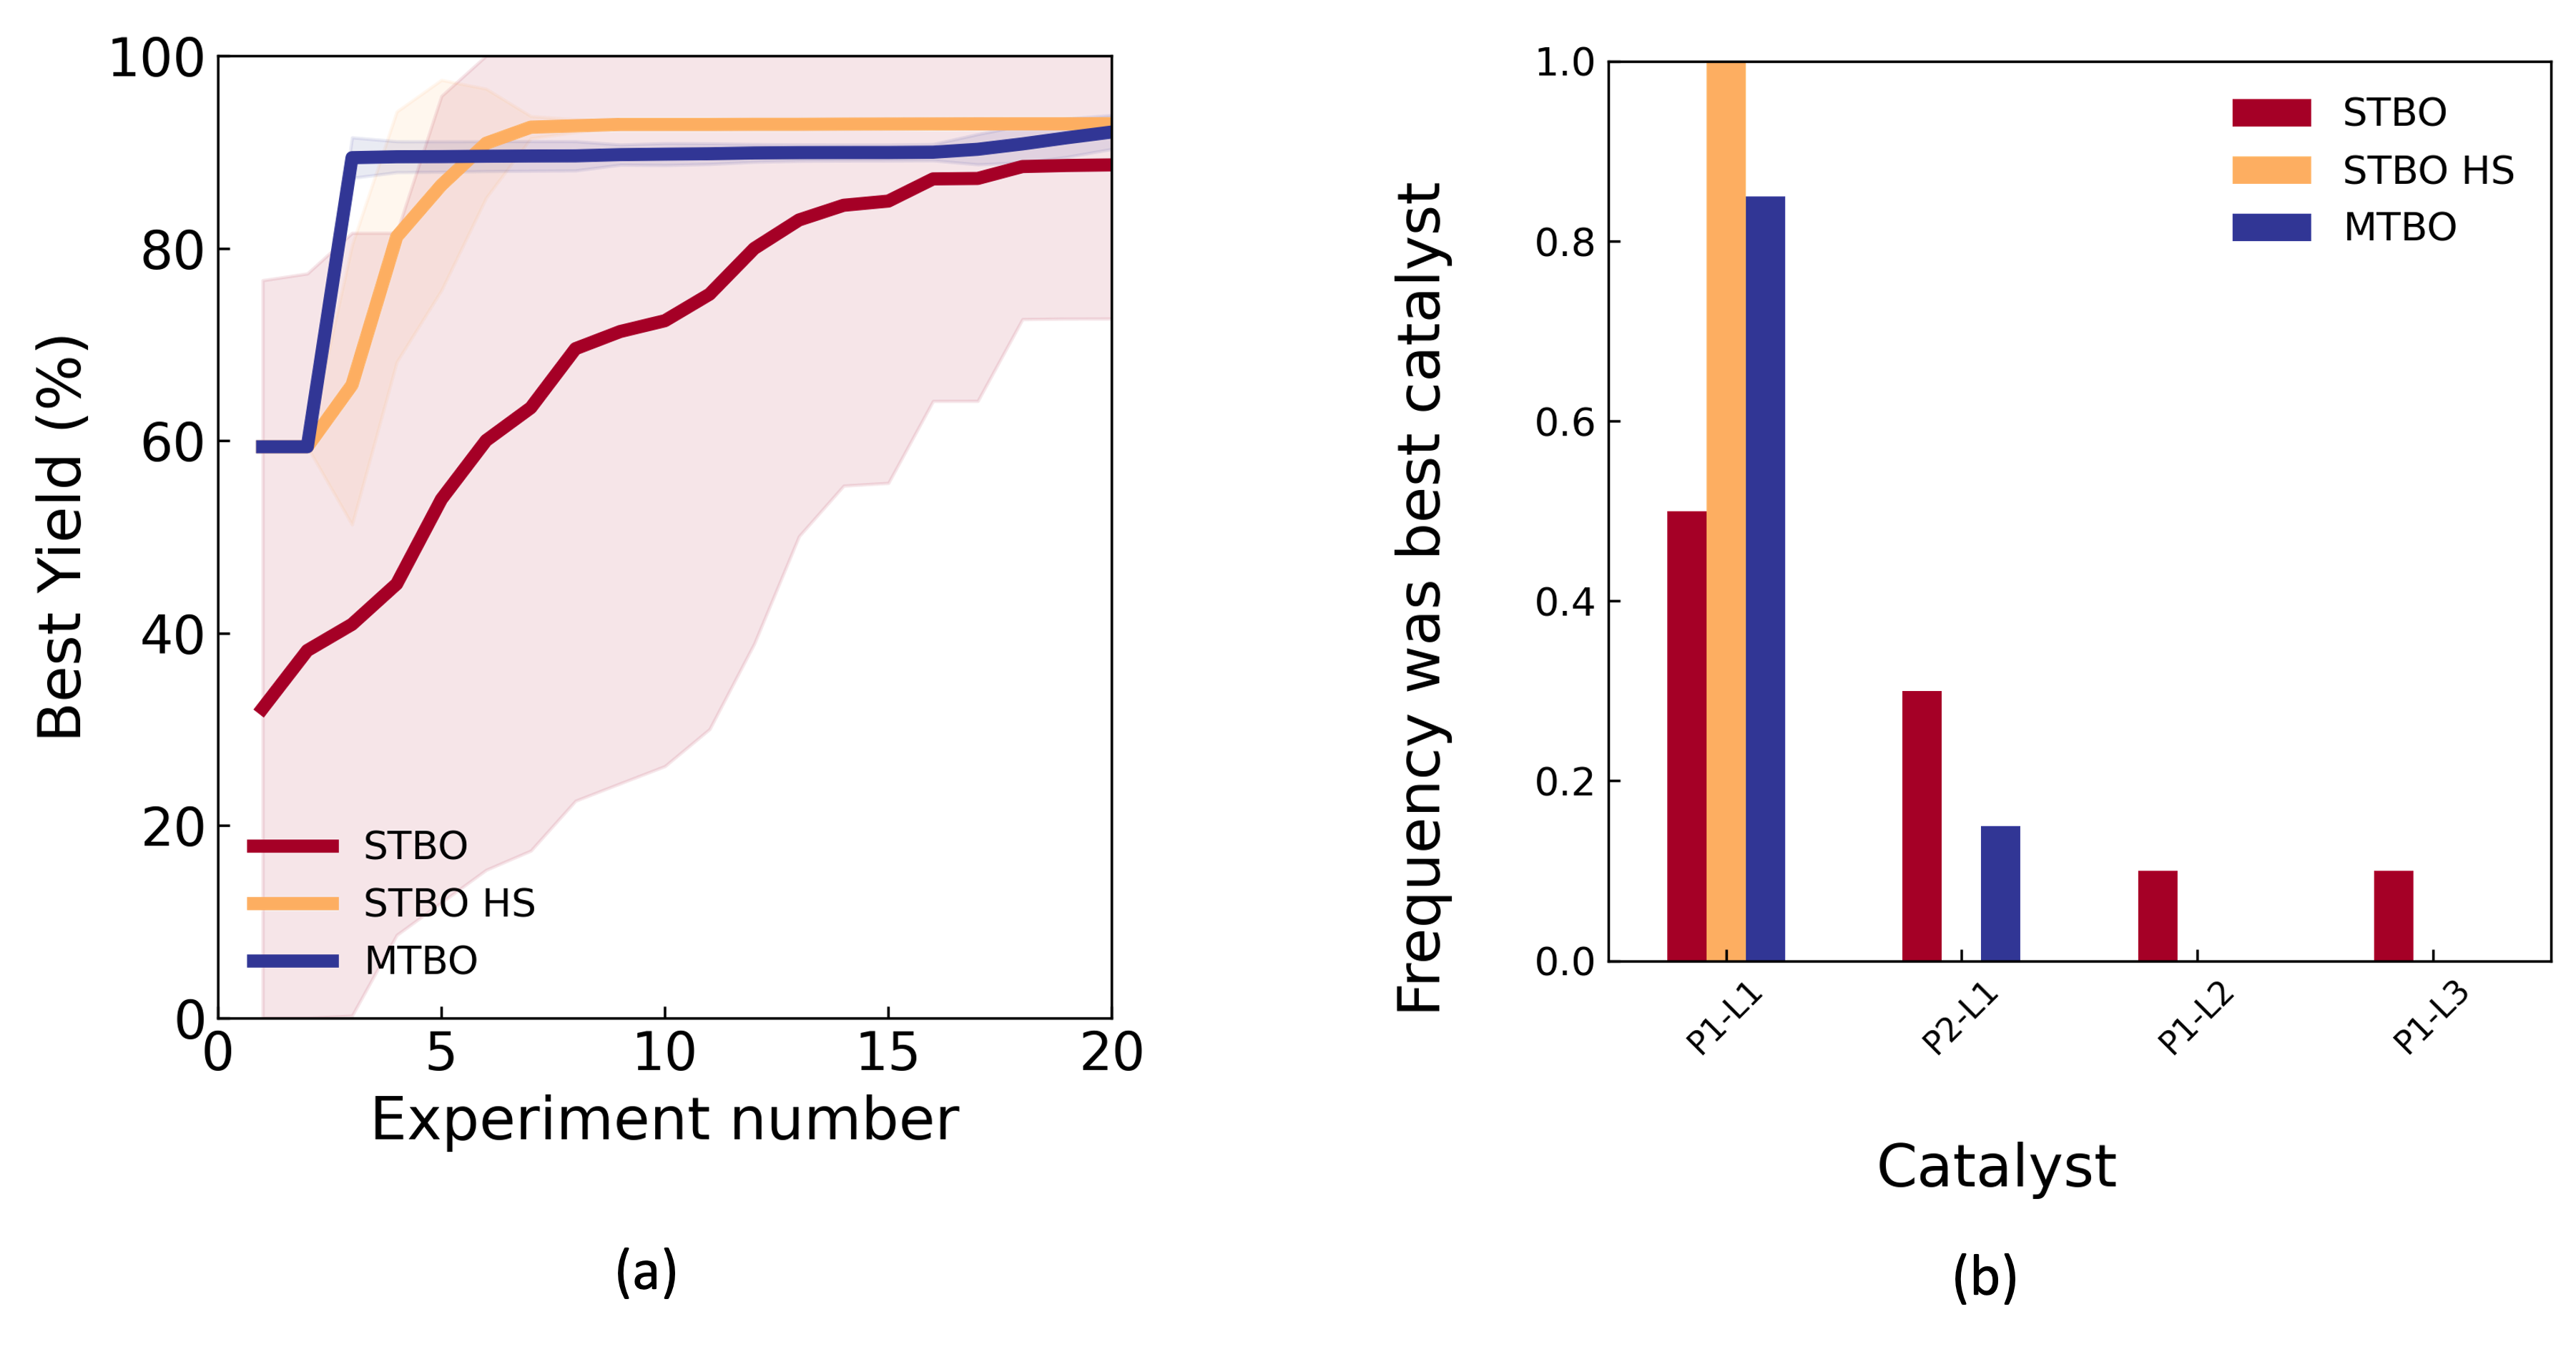
\includegraphics[width=\textwidth]{gfx/Chapter04/catalyst_optimization.png}

    \caption{A comparison of the performance of single-task Bayesian optimisation (STBO), STBO head start (STBO HS), and multi-task Bayesian optimisation (MTBO) of Suzuki B1 and all of Suzuki R1-R4 as auxiliary tasks. (a)  The average best yield with a 95 \% confidence interval over 20 repeats is shown.  (b) Frequency of selection of each catalyst in Scheme 1 by STBO and MTBO.}
    \label{fig:baumgartner_suzuki_reizman_suzuki_all_cotraining_optimisation}
\end{figure}

Here, STBO HS also performs well, suggesting that the optimal conditions from the auxiliary task are highly transferable to the new task. The success of STBO HS, however, shows that the similarity between tasks matters significantly for transfer learning.  

These simulated case studies suggest that the use of MTBO is often beneficial, particularly when not mapping the predicted reactivity differences of the main and auxiliary substrates \textit{a priori}. Initial guesses (optimisation starting points) are typically better than random initialization because of previous reaction information, and the rate of `best yield' improvement is also greater. In the best-case scenario, the reactivity of the new substrate is similar to those of previous datasets and results in a greater yield much faster than standard STBO. In the worst-case scenario, MTBO can fail with one noisy auxiliary case, but I found that using multiple auxiliary tasks helps to mitigate these issues.  With these findings, we were confident that MTBO would be effective in real-world case studies where we have experimental datasets from previous optimisation campaigns. Further \textit{in silico} case studies for other reaction types, namely Buchwald-Hartwig cross couplings, were also conducted and showed similarly promising results; these studies can be found in Appendix \ref{ch:benchmarking_appendix}.

\subsection{Experimental Case Studies: C-H Activation}

The reaction class that we targeted for our experimental MTBO study was the palladium-catalyzed C-H activation reaction, reported by Hennessy and Buchwald, yielding pharmaceutically relevant oxindoles  from their corresponding chloroacetanilides, as shown in Figure \ref{fig:ch_activation}. Each case study is highlighted if it is forming a potential bioactive fragment or active pharmaceutical ingredient (API) intermediate. The rationale behind these studies is two-fold: firstly, these oxindoles are closely related to many known bioactive molecules, and secondly, when considering optimal growth vectors for bioactive molecular fragments to grow into more potent drug candidates, the most beneficial transformations are often exploiting C--H bonds on the fragment to form new C--C bonds. Therefore, using MTBO, we aimed to rapidly optimize several transformations using different starting materials with unique functionalities to yield structurally diverse oxindole products by forming valuable sp\textsuperscript{2}-sp\textsuperscript{3} C--C bonds. Then, for future optimisation campaigns requiring oxindole syntheses, this model can be employed to expedite reaction optimisation and process development for new substrates.

\begin{figure}
    \centering
    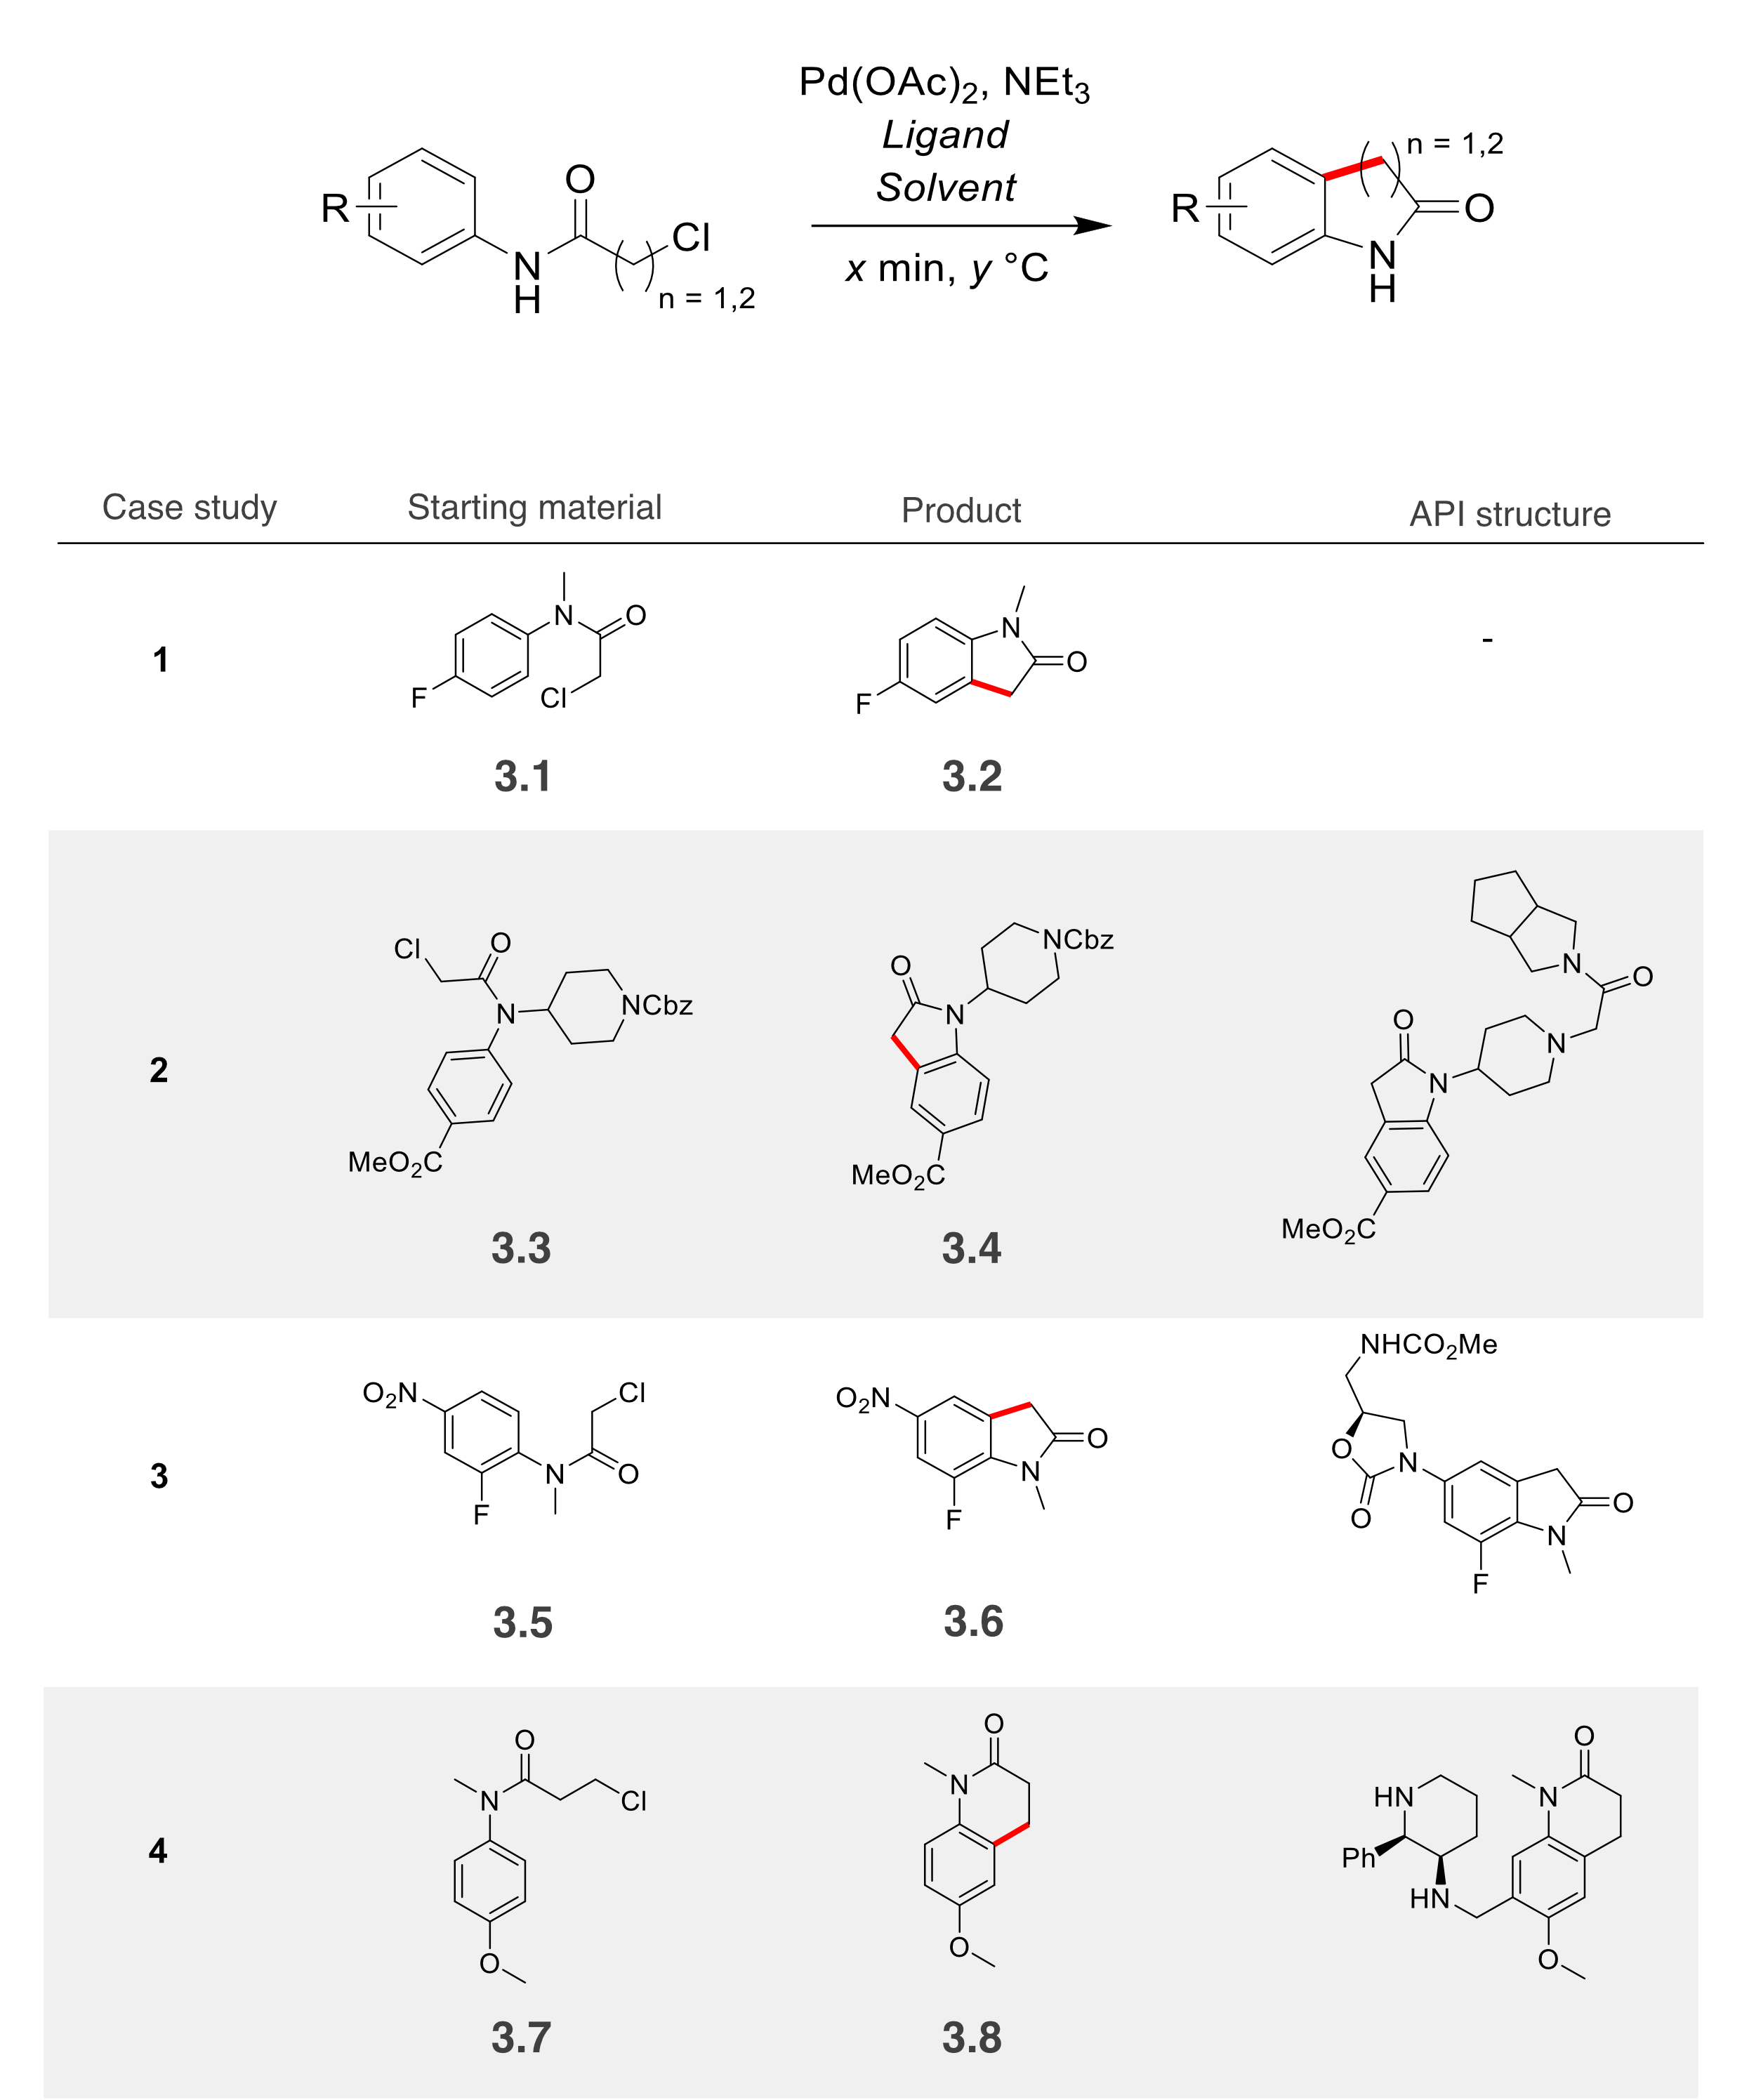
\includegraphics[width=\textwidth]{gfx/Chapter04/ch_activation_case_studies.png}
    \caption{ The reaction class of interest for the MTBO study, where the substituted chloroacetanilide, , reacts to form the corresponding oxindole. Pd(OAc)\textsubscript{2} and NEt\textsubscript{3} remain constant in each experiment, but the ligand, solvent, catalyst concentration, residence time and reaction temperature are optimized for each case study. Each experimental case study explored in this work, including the starting material used, the product formed and the API structure that the product is linked to.}
    \label{fig:ch_activation}
\end{figure}

For each case study, we optimized the continuous parameters: residence time (5 - 60 minutes), reaction temperature (50 - 150 °C) and catalyst concentration (1 - 10 mol\%), and the categorical parameters: solvent (toluene, DMA, acetonitrile, DMSO, NMP) and ligand (JohnPhos, SPhos, XPhos, DPEPhos), for the maximum product yield output. While it is possible to represent these categorical variables in numerous ways, the simplest representation (one-hot encoding) proved sufficient data to learn from. The first case study, utilized only single-task Bayesian optimisation (STBO) as there is no previous data to leverage model understanding for MTBO. The starting material reacts to form the molecular fragment (with potential growth vectors for further functionalization). The optimisation was initialized using 16 training experiments before the algorithm began to suggest experimental conditions. We subsequently optimized case study two, three and four with the experimental data from the previous case studies as separate tasks.

For each of these consecutive C-H activation case studies, iteratively fewer experiments were (generally) necessary to achieve an optimal set of reaction conditions for the highest process yields - this is illustrated in Figure \ref{fig:optimisation_curves}. This is because there was an increasing data-density that detailed optimal areas of parameter space for similar tasks (reactions of similar substrates), allowing for a progressively more efficient optimisation workflow. In each case study, only minimal amounts (for our specific reaction system) of starting materials were consumed to find optimal reaction conditions, which is very important in early-stage medicinal chemistry development applications when preservation of precious starting materials and speed of optimisation are paramount. Other common optimisation strategies, such as traditional one-factor at a time (OFAT) approaches, may provide modest process improvements in these scenarios but have been shown repeatedly to underperform when compared with statistical-based techniques. This methodology has therefore proven to be effective in real-world pharmaceutical applications for material- and cost-efficiency, with the bonus of full automation that allows scientists to use their human resource to focus on other areas of chemical development. Although these experimental studies focused on C--C bond formation by targeting C--H activation, these techniques can be utilized for other transformations to ultimately accelerate optimisation.

\begin{figure}
    \centering
    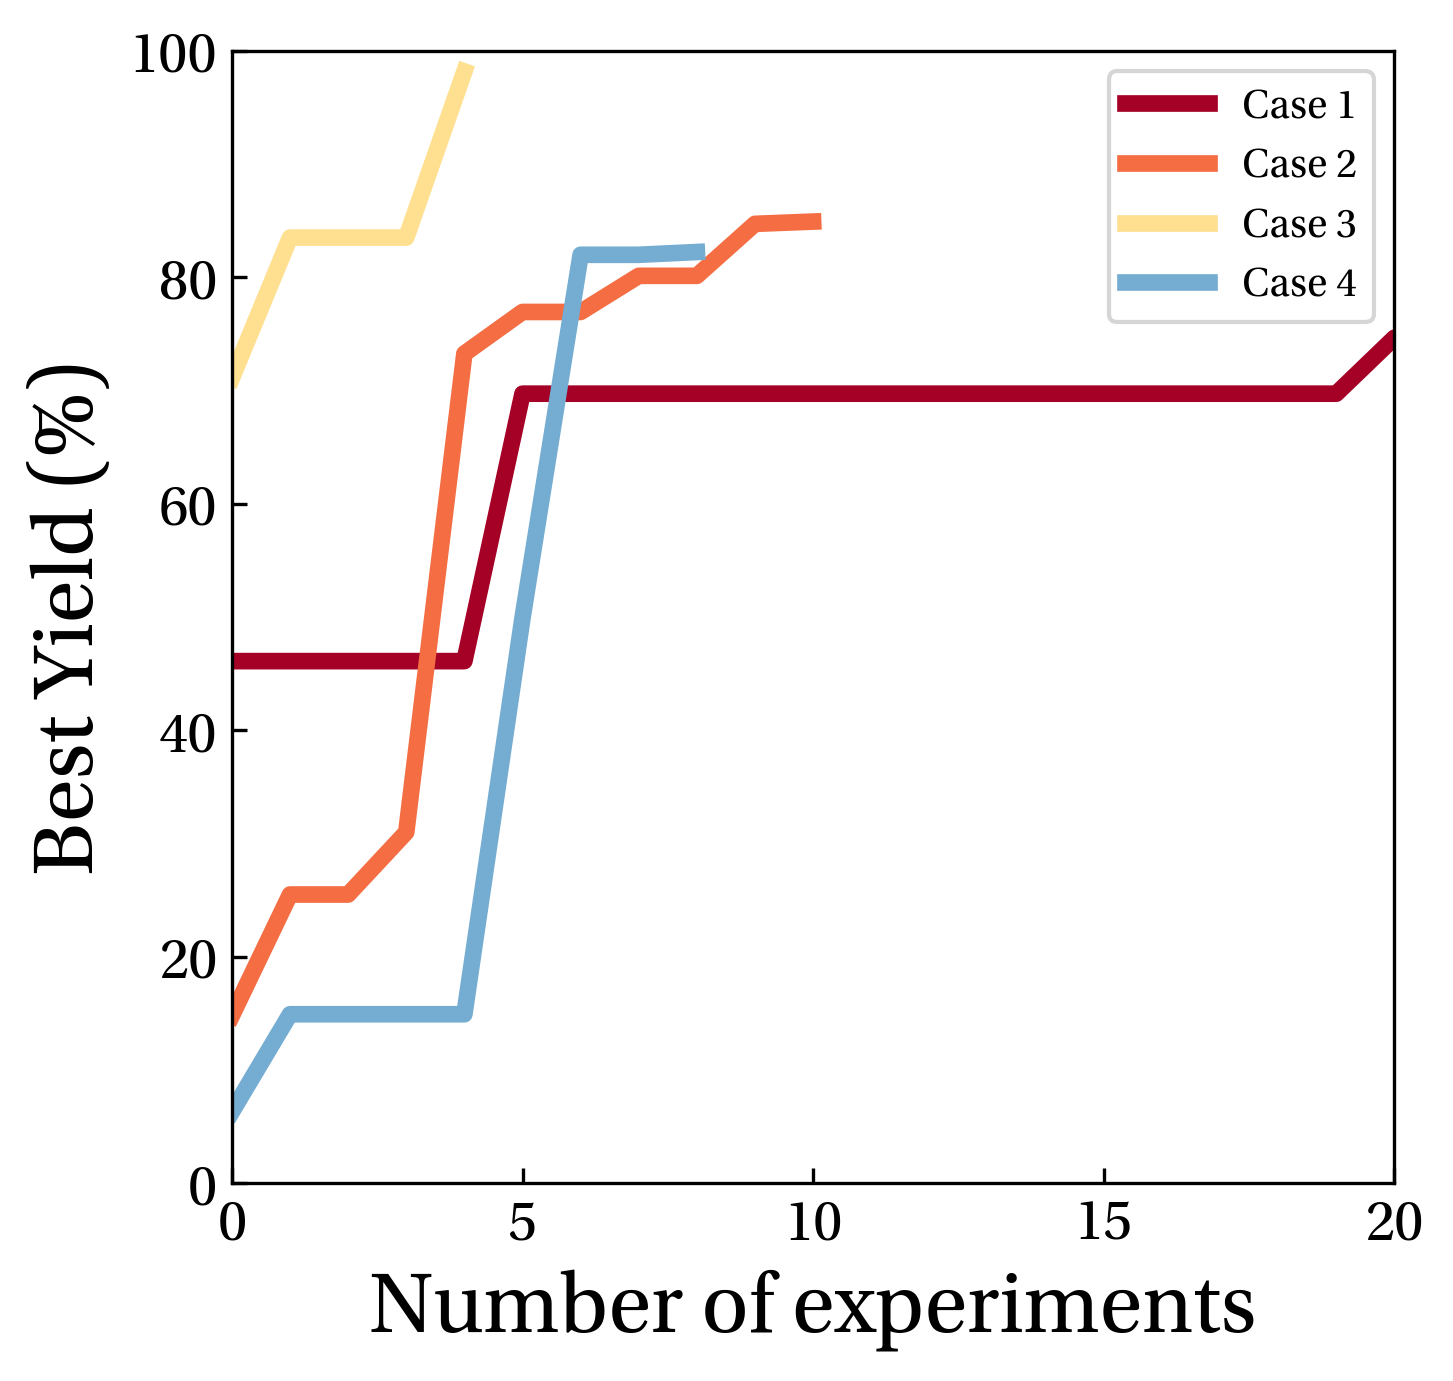
\includegraphics[width=0.7\textwidth]{gfx/Chapter04/ch_activation_optimization_curves.png}
    \caption{A plot of best yield of the products in each case study against the optimisation experimental number in each campaign.}
    \label{fig:optimisation_curves}
\end{figure}


\section{Conclusions}

The studies performed in this chapter, both \textit{in silico} and in real-world chemical applications, represent the first use of datasets from similar reactions to expedite current optimisation campaigns with multi-task Bayesian optimisation. This methodology drastically shortens optimisation timelines for pharmaceutically relevant transformations, whereas other traditional process optimisation techniques (i.e. design of experiments, kinetics studies) would require a significantly higher investment in starting materials, time and cost. This would likely make their optimisation infeasible in medicinal chemistry workflows and early-stage process development, unless using intuition-based optimisation techniques (such as OFAT) that are unlikely to obtain optimal results. By introducing more miniaturization technology, including smaller reactors/slugs and plate-based screening, there is the added opportunity to reduce material consumption even further using these automated platforms. 

The primary challenge when using multi-task Bayesian optimisation is its tendency to bias towards the best conditions found in a single auxiliary task, as shown in my \textit{in silico} studies. However, our results demonstrate that additional useful auxiliary tasks can reduce the impact of a noisy, low-yielding auxiliary task. Future work could use a more exploratory acquisition function in combination with the multi-task model to strike the right balance between biasing towards the auxiliary task data and exploring untested conditions.

The multi-task Bayesian optimisation algorithm used in this chapter is open-source and is released as a package within the Summit framework previously reported by our group. This step towards utilizing transfer learning for reaction optimisation will ultimately result in faster and more efficient optimisations, thereby serving as a broadly applicable enabling tool with relevance to early-stage process development, where industry-standard process optimisation techniques are impractical or even impossible to implement.


%*****************************************
%*****************************************
%*****************************************
%*****************************************
%*****************************************
